\section{Question 2}
\label{sec:q2}
\paragraph{\textbf{SQL query}}
First, we perform two sequential \mintinline{python}{DataFrame.crossJoin()} operations, each of them followed by a filtering operation to remove repetitions from the combination: this way, we obtained all the triples of vectors \(<X,Y,Z>\) in the dataset. Then, we compute the aggregate vectors for all the triples and compute the variance of those vectors. The chain of operations can easily be read from the following SQL query:
\begin{figure}[H]
\begin{minipage}{.6\textwidth}
\inputminted[fontsize=\footnotesize,]{sql}{../assets/code/q2.sql}
\end{minipage}
\begin{minipage}{.4\textwidth}
    \centering
    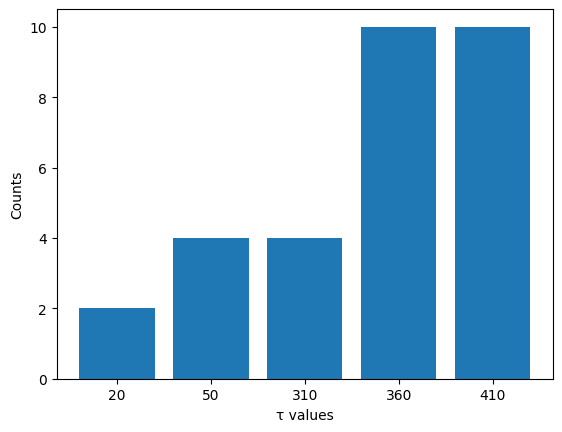
\includegraphics[width=.75\linewidth]{../assets/images/q2_results.png}
    \caption{Triples with aggregate variance $ \le \tau$}
    \label{fig:q2_results}
\end{minipage}
\end{figure}
The User Defined Function \mintinline{sql}{var_udf} in the query retrieves the vector corresponding to each id from the broadcasted map, computes the aggregate vector (component-wise summation of three vectors) and then computes the variance of the aggregate vector (\emph{aggregate variance}).

\paragraph{\textbf{Results}}
Our query took \textbf{237.11 seconds} to run on the cluster and the results are summarized in Fig.\ref{fig:q2_results}.

\begin{figure}[H]
    \begin{minipage}{.45\textwidth}
        \centering
        \begin{tabular}{l c}
    \toprule
    \textbf{Optimization} & \textbf{Execution time} \\
    \midrule
    All            & 163.56s    \\
    No numpy       & 443.19s    \\
    No repartition/coalesce  & 2108.38s     \\
    No broadcast   & ran out of heap    \\ 
    \bottomrule
\end{tabular}
\makeatletter\def\@captype{table}\makeatother% "Change float to table"
\caption{Impact of optimizations tricks on the dataset of size 125x10000, ran locally.}
\label{tab:q2_optimisations}
    \end{minipage}
    \hfill
    \begin{minipage}{.45\textwidth}
        \centering
        \begin{tabular}{l c}
    \toprule
    \textbf{Partitions} & \textbf{Execution time} \\
    \midrule
    32-64-128     & 237.11s    \\ 
    16-32-64      & 246.13s    \\ 
    64-128-256    & 295.03s    \\
    64-64-64      & 323.13s    \\
    \bottomrule
\end{tabular}
\makeatletter\def\@captype{table}\makeatother% "Change float to table"
\caption{Impact of partition combinations on the dataset of size 250x10000, ran on the server.}
\label{tab:q2_partitions}
    \end{minipage}
\end{figure}


\paragraph{\textbf{Optimization}}
The main indicator that we considered evaluating the performance of our SQL query was the \emph{execution time}. We leveraged a variety of techniques to improve it; their impact on performances is summarized in Tab.\ref{tab:q2_optimisations}. In the following, we are presenting the most relevant ones.
\begin{itemize}
    \item We broadcast the ID-values mapping to the worker nodes: this allows us to transfer only the IDs during the shuffle phases, severely reducing the network transfer speed bottleneck.
    \item We use the \mintinline{python}{.coalesce()} API to reduce the number of partitions after the two \mintinline{python}{.crossJoin()} operations; the number of partitions has been empirically fine-tuned (see Tab.\ref{tab:q2_partitions}).
    \item We use \mintinline{python}{numpy.ndarray}s instead of Python's built-in data types, as they provide better performances on mathematical operations; moreover, we were able to further improve the performances by reducing the size of the integer to 16 bits integers - which is the minimum size we could use before overflow issues would occur.
\end{itemize}
